%
% chapter.tex -- Homologie
%
% (c) 2021 Prof Dr Andreas Müller, Hochschule Rapperswil
%
\chapter{Homologie
\label{buch:chapter:homologie}}
\lhead{Homologie}
\rhead{}
Mit der Inzidenzmatrix war es möglich, einen Graphen zu beschreiben
und verschiedene interessante Eigenschaften desselben zu berechnen.
Damit können aber nur eindimensionale Strukturen analysiert werden:
Es ist zum Beispiel nicht möglich, ein Dreieck vom Rand eines
Dreiecks zu unterscheiden~\ref{buch:homologie:figure:zusammenziehbar}.
\begin{figure}
\centering
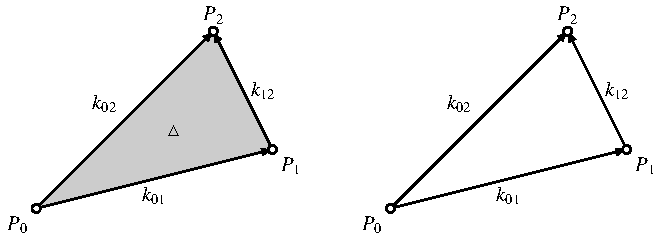
\includegraphics{chapters/95-homologie/images/dreieck.pdf}
\caption{Ein Dreieck $\triangle$ (rechts) und der Rand des Dreicks
(links) sind mit den Methoden
der Graphentheorie nicht unterschiedbar. 
Als topologische Räume sind das Dreieck und sein Rand aber ganz klar
unterschiedbar: In einem Dreieck ist jeder geschlossene Pfad in einen 
Punkt zusammenziehbar, aber die Randkurve ist nicht mehrzusammenziehbar,
sobald man das innere des Dreiecks entfernt.
\label{buch:homologie:figure:zusammenziehbar}}
\end{figure}
Die Randkurve ist in einem Dreieck zusammenziehbar, aber sobald man
das innere des Dreiecks entfernt, ist die Randkurve nicht mehr
zusammenziehbar.
Dreieck und der Rand des Dreiecks sind also grundsätzlich verschieden.

Die Inzidenzmatrix ordnet jeder Kante ihre beiden Endpunkte zu.
Die Homologietheorie verallgemeinert diese Idee.
Der sogenannte Randoperator ordnet jedem Dreieck, Tetraeder oder allgemein
jedem Simplex seinen Rand zu.
Damit wird es möglich, das Dreieck vom Rand des Dreiecks zu unterschieden.

%
% simplex.tex -- simplizes und simpliziale Komplexe
%
% (c) 2021 Prof Dr Andreas Müller, OST Ostschweizer Fachhochschule
%
\section{Simplexe und simpliziale Komplexe
\label{buch:section:simplexe}}
\rhead{Simplexe und simpliziale Komplexe}
Die Idee, das Dreieck und seinen Rand zu unterscheiden verlangt,
dass wir zunächst Dreiecke und deren höherdimensionale Verallgemeinerungen,
die sogenannten Simplizes entwickeln müssen.

\subsection{Simplexe und Rand
\label{buch:subsection:simplexe}}

\subsubsection{Rand eines Dreiecks}
Die Inzidenz-Matrix eines Graphen hat einer Kante die beiden Endpunkte
mit verschiedenen Vorzeichen zugeordnet.
Dieses Idee soll jetzt verallgemeinert werden.
Der Rand des Dreiecks $\triangle$ in
Abbildung~\ref{buch:homologie:figure:zusammenziehbar}
besteht aus den Kanten $P_0P_1$, $P_1P_2$ und $P_0P_2$.
Für eine algebraische Definition müssen die Kanten offenbar eine
Orientierung haben, die ist aber garantiert, da wir den Anfangs-
und Endpunkten einer Kante verschiedene Vorzeichen gegeben haben.
Dem Dreieck $\triangle$ werden dann die drei Kanten $k_{01}$, $k_{02}$
und $k_{12}$ zuogeordnet, aber mit zusätzlichen Vorzeichen, die
die Orientierung festhalten.
Durchläuft man den Rand von $\triangle$ in der Reihenfolge $P_0P_1P_2$,
dann müssen die Kanten $k_{12}$ und $k_{02}$ ein negatives Vorzeichen
erhalten.

Wir können diese Zuordnung wieder mit einer Matrix ausdrücken.
\[
\begin{matrix}
\text{$k_{01}$:}\mathstrut\\
\text{$k_{02}$:}\mathstrut\\
\text{$k_{12}$:}\mathstrut
\end{matrix}
\qquad
\partial
=
\begin{pmatrix*}[r]
1\mathstrut\\
-1\mathstrut\\
1\mathstrut
\end{pmatrix*}
\]

\subsubsection{Simplizes}
Punkte, Kanten und Dreiecke sind die einfachsten Fälle sogenannter
Simplizes.
Wir formulieren die Definition dieser Objekte auf eine Weise,
die uns ermöglichen soll, sie auf beliebige Dimension zu verallgemeinern.

Die Strecke, die die Punkte $P$ und $Q$ miteinander verbindet,
kann beschrieben werden durch eine Parametrisierung
der Form
\begin{equation}
s_1
\colon
t
\mapsto
t\vec{p} + (1-t) \vec{q}
=
t_0 \vec{p} + t_1\vec{q},
\end{equation}
wobei die beiden positiven reellen Zahlen $t_0,t_1\in\mathbb{R}$ die
Bedingung $t_0 + t_1 = 1$ erfüllen.
Für ein eindimensionales Objekt brauchen wir also zwei Punkte und zwei
positive Parameter, die sich zu $1$ summieren.
Die Mengen $\triangle_1=\{ (t_0,t_1)\,|t_i\ge 0, t_0+t_1=1\}$ kann also
ganz allgemein als Parameterraum zur Beschreibung eindimensionalen Objektes
mit den Endpunkten dienen.
Eine Strecke ist also eine Abbildung der Form
\begin{equation}
s_1
\colon
\triangle_1 \to \mathbb{R}^N
:
(t_0,t_1)
\mapsto
t_0 \vec{p} + t_1\vec{q},
\end{equation}
und der Rand besteht aus den Punkten $s_1(0)$ und $s_1(1)$, wobei der
Anfangspunkt $s_1(0)$ mit einem negativen Vorzeichen versehen wird.

Für höhere Dimensionen brauchen wir auf analoge Weise erst wieder einen
geeigneten Parameterraum.
Die Menge
\[
\triangle_n
=
\{(t_0,\dots,t_n)\in\mathbb{R}^{n+1}\,|\, t_i\ge 0,t_0+t_1+\dots+t_n=1\}
\]
beschreibt zum Beispiel für $n=2$ ein Dreieck und für $n=3$ ein 
Tetraeder.

Gegeben $n+1$-Punkte $P_0,\dots,P_n$ mit Ortsvektoren
$\vec{p}_0,\dots,\vec{p}_n$ können wir eine Abbildung
\begin{equation}
s_n
\colon
\triangle_n
\to
\mathbb{R}^N
:
(t_0,\dots,t_n)
\mapsto
t_0\vec{p}_0
+
t_1\vec{p}_1
+
\dots
+
t_n\vec{p}_n
\end{equation}
Eine solche Abbildung verallgemeinert also den Begriff einer Strecke
auf höhere Dimensionen.

\begin{definition}
\label{buch:def:simplex}
Ein $n$-dimensionales {\em Simplex} oder {\em $n$-Simplex} ist eine
stetige Abbildung $s_n\colon\triangle_n\to X$.
\end{definition}

Die Ecken des $n$-Simplex $\triangle_n$ sind die Standardbasisvektoren
in $\mathbb{R}^{n+1}$.
Mit $e_k$ bezeichnen wird die Ecke, deren Koordinaten $t_i=0$ sind für 
$k\ne i$, ausser der Koordinaten $t_k$, die den Wert $t_k=1$ hat.

\subsubsection{Rechnen mit Simplizes}
Damit wir leichter mit Simplizes rechnen können, betrachten wir
jedes Simplex als einen Basisvektor eines abstrakten Vektorraumes.
Zu einem $n$-Simplex gehören Vektorräume $C_l$ für jede Dimension
$l=0$ bis $l=n$.
Der Vektorraum $C_0$ besteht aus Linearkombinationen
\[
C_0 
=
\{ x_0 P_0 + \dots + x_n P_n \,| x_i\in\mathbb{R} \},
\]
$C_0$ ist ein $n$-dimensionaler Raum.
Der Vektorraum $C_1$ besteht aus Linearkombinationen der Kanten
\[
C_1 
=
\biggl\{
\sum_{i<j}
x_{ij} k_{ij}
\,
\bigg|
\,
x_{ij}\in\mathbb{R}
\biggr\},
\]
wobei $k_{ij}$ die Kante von der Ecke $i$ zur Ecke $j$ ist.

In Dimension $l$ bezeichnen wir mit $C_l$  den Vektorraum bestehend
aus den Linearkombinationen
\[
C_l
=
\biggl\{
\sum_{i_1<\dots<i_l} x_{i_1\dots i_l} s_{i_1\dots i_l}
\,
\bigg|
\,
s_{i_1\dots i_l}\in\mathbb{R}
\biggr\},
\]
wobei $s_{i_1\dots i_l}$ das Simplex mit den Ecken $i_1,\dots,i_l$ ist.

Für $n=1$ gibt ist $C_1$ ein eindimensionaler Vektorraum und $C_0$
ist zweidimensional.
Die Randabbildung, die einer Kante den Rand zuordnet, ist
\[
\partial
\colon 
C_1\to C_0
:
s_{01}
\mapsto
1\cdot s_0 + (-1)\cdot s_1
\]
und hat in den oben beschriebenden Basen die Matrix
\[
\partial 
=
\begin{pmatrix}
1\\
-1
\end{pmatrix}.
\]

\subsubsection{Rand eines Simplex}
Einem Simplex muss auch der Rand zugeordnet werden können.
Setzt man in $\triangle_2$ den Parameter $t_k=0$, dann erhält
man die Kante,
die der Ecke mit Nummer $k$ gegenüberliegt.
Für jedes $k$ gibt es also eine Abbildung
\[
i_k
\colon
\triangle_{n-1} \to \triangle_n
:
(t_0,\dots,t_n)
\mapsto
(t_0,\dots,t_{k-1},0,t_{k},\dots,t_n),
\]
in die Kante gegenüber der Ecke $e_k$.
Dies ist auch die Art, wie Kanten des Dreiecks $\triangle$ 
in Abbildung~\ref{buch:homologie:figure:zusammenziehbar}
orientiert wurden.

Für den Rand des $2$-Simplexes mussten die Kanten mit alternierenden
Vorzeichen zugeordnet werden.
Damit wird erreicht, dass jeder Punkt sowohl Endpunkt einer 
Kante und
ausserdem Anfangspunkt der nächsten Kannte ist.
Diese Eigenschaft soll auch in höheren Dimensionen erhalten bleiben.
Die vier Dreiecke, die den Rand eines $3$-Simplex ausmachen,
müssen so orientiert werden,
dass jede Kante in beiden Richtungen durchlaufen wird.

\begin{definition}
\label{buch:def:randoperator}
Der Randoperator ordnet die Kanten eines $n$-Simplex mit alternierenden
Vorzeichen zu, die Matrix ist
\[
\]
\end{definition}


\subsection{Triangulation
\label{buch:subsection:}}



%
% komplex.tex -- simpliziale Komplexe und Kettenkomplexe
%
% (c) 2021 Prof Dr Andreas Müller, OST Ostschweizer Fachhochschule
%
\section{Kettenkomplexe
\label{buch:section:komplex}}
\rhead{Kettenkomplexe}

\subsection{Randoperator von Simplexen
\label{buch:subsection:randoperator-von-simplexen}}

\subsection{Kettenkomplexe und Morphismen
\label{buch:subsection:kettenkomplex}}

%
% homologie.tex -- Homologie eines Komplexes
%
% (c) 2021 Prof Dr Andreas Müller, Hochschule Rapperswil
%
\section{Homologie
\label{buch:section:homologie}}
\rhead{Homologie}

\subsection{Homologie eines Kettenkomplexes
\label{buch:subsection:homologie-eines-kettenkomplexes}}

\subsection{Induzierte Abbildung
\label{buch:subsection:induzierte-abbildung}}

\subsection{Homologie eines simplizialen Komplexes
\label{buch:subsection:simplizialekomplexe}}


%
% mayervietoris.tex
%
% (c) 2021 Prof Dr Andreas Müller, OST Ostschweizer Fachhochschule
%
\section{Exaktheit und die Mayer-Vietoris-Folge
\label{buch:section:mayervietoris}}
\rhead{Exaktheit und die Mayer-Vietoris-Folge}
Die Berechnung der Homologie-Gruppen ist zwar im Wesentlichen ein 
kombinatorisches Problem, trotzdem ist eher aufwändig.
Oft weiss man, wie sich toplogische Räume aus einfacheren Räumen
zusammensetzen lassen.
Eine Mannigkfaltigkeit zum Beispiel wird durch die Karten
definiert, also zusammenziehbare Teilmengen von $\mathbb{R}^n$,
die die Mannigkfaltigkeit überdecken.
Das Ziel dieses Abschnittes ist, Regeln zusammenzustellen, mit denen
man die Homologie eines solchen zusammengesetzten Raumes aus der
Homologie der einzelnen Teile und aus den ``Verklebungsabbildungen'',
die die Teile verbinden, zu berechnen.

\subsection{Kurze exakte Folgen von Kettenkomplexen
\label{buch:subsection:exaktefolgen}}

\subsection{Schlangenlemma und lange exakte Folgen
\label{buch:subsection:schlangenlemma}}

\subsection{Mayer-Vietoris-Folge
\label{buch:subsection:mayervietoris}}

%
% fixpunkte.tex
%
% (c) 2021 Prof Dr Andreas Müller, OST Ostschweizer Fachhochschule
%
\section{Fixpunkte
\label{buch:section:fixpunkte}}
\rhead{Fixpunkte}
Zu jeder Abbildung $f\colon X\to X$ eines topologischen Raumes in sich
selbst gehört die zugehörige lineare Abbildung $f_*\colon H_*(X)\to H_*(X)$
der Homologiegruppen.
Diese linearen Abbildungen sind im Allgemeinen viel einfacher zu
analysieren.
Zum Beispiel soll in Abschnitt~\ref{buch:subsection:lefshetz}
die Lefshetz-Spurformel abgeleitet werden, die eine Aussagen darüber
ermöglicht, ob eine Abbildung einen Fixpunkt haben kann.
In Abschnitt~\ref{buch:subsection:brower} wird gezeigt wie man damit 
den Browerschen Fixpunktsatz beweisen kann, der besagt, dass jede
Abbildung eines Einheitsballs in sich selbst immer einen Fixpunkt hat.

\subsection{Lefshetz-Spurformel
\label{buch:subsection:lefshetz}}

\subsection{Brower-Fixpunktsatz
\label{buch:subsection:brower}}








